% This is sample paper.tex, a sample chapter demonstrating the
% LLNCS macro package for Springer Computer Science proceedings;
% Version 2.20 of 2017/10/04
%
\documentclass[runningheads]{llncs}
%
\usepackage{graphicx}
\usepackage{caption}
\usepackage{refstyle}
\graphicspath{ {./images/} }
% Used for displaying a sample figure. If possible, figure files should
% be included in EPS format.
%
% If you use the hyperref package, please uncomment the following line
% to display URLs in blue roman font according to Springer's eBook style:
% \renewcommand\UrlFont{\color{blue}\rmfamily}

\begin{document}
%
\title{Information System Prototyping\thanks{Supported by RWTH Aachen}}
%
%\titlerunning{Abbreviated paper title}
% If the paper title is too long for the running head, you can set
% an abbreviated paper title here
%
\author{Felix Voigtländer\inst{1}}
%
%\authorrunning{F. Voigtländer}
% First names are abbreviated in the running head.
% If there are more than two authors, 'et al.' is used.
%
\institute{RWTH Aachen, Aachen 52062, Germany}
%
\maketitle              % typeset the header of the contribution
%
\begin{abstract}
  %TODO
This paper explores the implications of the use of prototyping and rapid prototyping.
It explains the issues with conventional methodologies, such as the waterfall model.
Then we explain what prototypes are and what prototyping means, which we'll discuss.
To address the difficulty of managing projects using prototypes the Agile approach
to software development is explained, of which its model Kanban is detailed.
Finally, an example is given and the paper is concluded.

\keywords{Prototyping \and Rapid Prototyping \and Agile \and Kanban \and User Interface}
\end{abstract}
%
%
%
\section{Introduction}
Traditional software methodologies have many issues such as unsatisfied customers,
minimal and late user involvement during development, and long development cycles resulting
in high development costs.

Prototyping is a tool that addresses these issues and has been effective and efficient
in software development, especially in the context of user interface design.

This paper addresses the issues of conventional methodologies, explains prototypes and prototyping,
discusses the advantages and disadvantages of the use of prototyping, the issue of the difficulty in
managing projects using the prototyping approach is addressed with the agile methodology
and its Models of which the Kanban model is explained in greater detail,
then an example is given and finally summarizes the use of prototyping and rapid prototyping.

\section{Issues of traditional methodologies}
Traditional methodologies such as the waterfall model \cite{ref_waterfall} 
are simple to understand approaches to software development, which makes it 
easy to manage. All stages are clearly defined and a detailed design document
reduces the risk of feature creep and increased development time and cost.
Due to the static general terms and conditions set at the beginning of the Project
production can be efficient and predictable while reducing waste, unnecessary features,
and content.

Yet, these models do not offer flexibility to changing requirements and due to the tendency of 
traditional models for long development cycles user feedback can only be gathered at the end 
of projects \cite{ref_health} increasing the time and cost of further 
alterations. Especially when complex factors are involved, such as human-machine interaction,
it becomes problematic to make predictions in conventional methodologies \cite{ref_RPalternativeStrategy}. 
The mutual understanding of the vision of a project is also not ensured in traditional approaches, 
since as \cite{ref_RPalternativeStrategy}
puts it "Clients don't know their requirements until the see them implemented"

Therefore conventional methodologies do not offer satisfactory results \cite{ref_RPalternativeStrategy}.
These approaches do not reduce development time and cost, yield unsatisfied costumers,
even with extensive documentation communication problems are not reduced and there is 
no guarantee that the right product is produced \cite{ref_RPalternativeStrategy}.

\section{Prototypes}
A prototype is \cite[a working model of (parts of) an information system, 
which emphasizes specific aspects of that system]{ref_prac}. These Prototypes
are unfinished, but represent the vision of the final product and may vary depending 
on the state and needs of a project. Prototypes may evolve through iteration into the final product or
throwaway prototypes may be discarded after their use. Low-technology prototypes such as the use of post-it 
notes or flip-charts may also be used, which empower the user to alter prototypes 
without any kind of technical-knowledge \cite{ref_prac}. 

Prototypes may be categorized into horizontal and vertical prototypes, in which
horizontal prototypes summarize the incomplete development of most system functions,
while vertical prototypes include selected complete features or system functions.
Incremental prototypes involve a series of horizontal and vertical moves \cite{ref_prac}.

Prototypes may also be distinguished via their functionality. 
Visual prototypes display the "look and feel" of the final product, but might have little 
to no functionality \cite{ref_RPInAction}. These are often used at the beginning of a project and to iterate 
user interfaces and are used as a reference for the final product, but are ultimately thrown away.
On the other hand, we have executable prototypes, which are useable and often evolve into the final product.
Executable prototypes may also be used to explore new functionalities and to test their feasibility\cite{ref_RPInAction}.

Another form of classification for prototypes are Floyd's 3"E"s.
Exploratory prototypes are used to evaluate requirements and their potential solution. Such prototypes can be functional and 
visual prototypes.
Experimental prototypes involve the implementation of selected requirements and features. Their evaluation result in the feasibility
and suitability of the implemented features.
Lastly, evolutionary prototypes evolve into the final product and adapt to changing requirements. Such prototypes may also be used for
pilot systems \cite{ref_ui}.

In a nutshell, many kinds of prototypes can be used to fit the needs of the project at hand.

\section{Prototyping}
Prototyping is the simple procedure of using prototypes during the project, which should be combined with others\cite{ref_prac}. 
During prototyping models of the product are shown to the user or customer, which are then discussed to evaluate problems 
and further advancements. Prototyping can be used when requirements are unclear especially with systems with high user interaction 
or systems require a higher form of cognitive processing from users such as "soft-skills".
The use of prototypes also helps the communication between everyone involved in the project, serving as a reference for everyone 
involved \cite{ref_RPInAction}.

The use of prototyping may require media which makes prototyping efficient and effective. Such tools need to offer modularity and plasticity.
Modularity enables the developer to add, remove, and alter modules, without causing many issues in other systems. Plasticity allows alterations
without significant time and cost penalties \cite{ref_RPalternativeStrategy}. The Rapid synthesis of prototypes is also useful with the use of 
prototypes\cite{ref_RPalternativeStrategy}. To ensure stability throughout many iterations during the project a layered approach may be 
used as well \cite{ref_health}.

A special form or prototyping is rapid prototyping(RP). RP acknowledges the complexity of aspects in development, rather than trying to minimize 
the complexity. This methodology expects that the first approach is probably faulty, but iterates and improves the product with the discovery of
problems. The goal of RP is to minimize the issues related to traditional development approaches like the waterfall model \cite{ref_RPalternativeStrategy}.


\section{Current State}
A study by the Philipps-University Marburg \cite{ref_health} used an application framework and
rapid application development approach for their information system in healthcare.
Lenz and Kuhn\cite{ref_health} explain that traditional information system development approaches, like
the waterfall model, are inadequate for RAD since they do not consider requirement changes during development. 
Traditional software engineering methods also tend to long development cycles, thus late feedback from users.

To apply rapid prototyping to huge healthcare information systems while maintaining flexibility and stability
a layered approach to system evolution with the addition of a generator-tool for application development 
have been used. 

The paper describes the disadvantages of heterogeneous databases and modules, due to module integration
from different developers, and bugs in lower layers causing complex and hard to debug issues in higher layers, 
for which smaller and robust core systems for future systems are proposed. Yet, prototyping yielded 
satisfactory results with high quality.

Another study by Jones and Richey \cite{ref_RPInAction} investigated the use of rapid prototyping for 
two projects in instructional design by designers and customers. 

The projects showed the production of two products of high quality in a short period. The customer
was involved in the first project and was satisfied with its results. Tasks could be completed concurrently
and collaboratively, which is not possible with the linear approach of conventional methods.

The paper concluded, that projects created using the Rapid Prototyping methodologies created useable products, that were 
delivered in a shorter time, and were received by satisfied customers. Rapid Prototyping appears to provide one solution 
to produce high-quality products in less time.

In a nutshell, both papers concluded that the use of prototyping yielded satisfying results with high quality, with low
development time and costs, if the known issues of prototyping have been addressed correctly.

\section{Benefits and Problems with Prototyping}
Prototyping as well as Rapid Prototyping(RP) aim to reduce the issues related to conventional development methodologies. Prototyping
benefits the communication and solves communication problems across the team, customers and users\cite{ref_RPalternativeStrategy} serving as a reference point already 
early and during development\cite{ref_prac}. The customer is left satisfied, by being able to be involved during the development 
and can help with feedback to produce a better product. Also a tendency of customers and users buying into prototypes result in a greater
commitment in a project. Due to the discussion of prototypes, requirements are better outlined from all parties involved causing the reduction
of unnecessary requirements and features, cutting cost and development time \cite{ref_prac}. Due to adjusted requirements, 
late alterations with high development times and costs are avoided and found early in development instead.

Yet, continual user participation and its rapidity may become stressful for developers, which might need additional skills and knowledge about
prototyping tools. Early user involvement might oversell the final product leading to the creation of unrealistic requirements, making it harder 
to manage user expectations. Larger systems are difficult to prototype since the complete infrastructure needs to be set up first\cite{ref_prac}.

Projects using prototyping become harder to manage. Due to throwaway prototypes the cost of the development effort is increased 
and due to creeping scopes\cite{ref_featurecreep} the project becomes difficult to budget and may result in longer development cycles. 
The use of prototypes may also result in a design-by-repair approach and may reduce creativity due to developers buying into one 
prototype instead of finding a better solution.

\section{The Agile Methodology}
To address the issues with the management of a project using the prototyping approach different methodologies other than 
conventional methodologies, like the waterfall model, need to be used. A promising approach is the "agile" approach
to project management. It can be used in combination with prototyping.

The most important thing to note is that agile is not defined by tools, models, or a framework, but rather by a mindset\cite{ref_agilemanifesto}. 
This mindset consists  of its values and principles, which helps on how to approach a project, it relies on the collaboration 
in teams and the flow of information. Agile is also customer-centric and puts him as part of the development team. Yet to 
give the mindset a structure and to ease the flow of information agile practices and models may be used.

This mindset is set by the Agile Manifesto\cite{ref_agilemanifesto}, which specifies its values:
\begin{enumerate}
  \item Individuals and interactions over processes and tools
  \item Working software over comprehensive documentation
  \item Customer collaboration over contract negotiation
  \item Responding to change over following a plan 
\end{enumerate}
Such values address the issues coming from prototyping. It emphasizes the collaboration of teams and customers, working software
and responding to change, while ignoring the use of processes, tools, documentation, contract negotiation and following a plan.

Team collaboration is at the forefront of agile development, thus it is about communication and working together. 
Finding problems together and solving problems together. This is valued more than using tools and processes, which are be rigid and outdated
and thus cannot react effective and efficient enough to a changing development environment.

Producing working software and prototypes to gain direct feedback from customers or consumers to finding problems early on,
which might have been unknown during the planning stages of development. In case of issues alterations are less costly to implement, 
since less systems rely on newly implemented systems. This is valued more than comprehensive documentation, which might become outdated, 
imprecise and faulty. With the value being set, systems can be structured accordingly, as example in \cite{ref_health}, to address
issues of instability from many iterations.

With the use of early working prototypes, the customer can give direct feedback early on, simplifying changes which are easy to adapt,
leading to greater customer satisfaction and more predictable software development timelines. This is valued more than extensive 
contract negotiations with the customers at the start of the project, which become outdated to which the customer is stuck and might 
be unsatisfied with or result in revisions late in development with higher development cost and time.

It is more efficient and cost-effective to respond to change and to adapt instead of following an outdated plan, which might even be faulty.

To summarize, the agile methodology is a mindset for software development. It is outlined by its values\cite{ref_agilemanifesto}
which should be seen as guidelines, rather than rules to follow.

\section{Kanban Methodology}
To give the mindset of the agile approach to software development a structure and to make it easier to use, agile methods might 
be applied. These incorporate the values and principles of agile software development. Each method can be adjusted to fit the 
needs of the team or the project to be as effective as possible. 
Further changes to models can be implemented at any time to improve it. Here are some examples of agile methods:

\begin{enumerate}
  \item SCRUM is a framework which uses an iterative, incremental approach, which is self-improving through reviews and self-reflection. 
  Thus it is flexible and adaptive and aims to improve the development cycle by periodic reevaluations. This makes it also more 
  effective and gradually increases quality.
  \item Extreme Programming (XP) is for changing or unknown requirements in a project for small to medium-sized teams. It also consists
  of lots of testing and pair programming.
  \item Kanban is a visual management method separated into different sections for parallel tasks with a task limit per section. The model 
  shows bottlenecks and is self-improving. This method will be elaborated later on.
\end{enumerate}

This paper explains the Kanban methodology in greater detail. Kanban was developed by Taiichi Ohno in 1940 for Toyota in Japan \cite{ref_kanban}. 
It aimed to be a simple framework for managing tasks and inventory for every stage in automotive production. The goal of this model 
was to improve productivity compared to American rivals and to avoid bottlenecks and over-stocking during production. 

Kanban is a tool for visualizing workflow and managing it. It limits work in progress, improves the flow of parallel tasks in its development 
and is a great tool for teams to self manage. This model does not force organizational, structural, or process changes, instead change happens 
iteratively and slowly for the team to adapt to.

For the visualization, a board with successive sections and tasks are used. The board can be a physical board with post-it notes or an electric board like Trello. 

The Tasks move from one section to another according to their state. These Tasks may be features, changes or even bug fixes, which should be 
manageable by one person. 

Sections may have different policies, for example a definition of done, thus which criteria need to be met for a task to move on. All Sections
have a maximum number of tasks which they can hold, once a section reaches its maximum number of tasks no tasks are allowed to be moved to 
this section. The section must be freed up by completing its tasks and moving them on.

Each iteration can be a week or a month, with the preference for smaller timescales. In each iteration tasks may be selected, 
which should be completed by the end of the iteration. It is advantageous to select tasks, which result together in working software or prototypes.

The main goal of this model is to improve the flow of information and to ensure a steady workflow without bottlenecks. Thus the board should 
be easy to read and understandable. 

A basic structure of this model, see \figref{kanban}, consists of the following sections, which will be explained in detail: 
backlog, todo, in progress, and done. Naming, the number of sections and structure may be changed to better suit the team.

\begin{figure}[!htb]
  \centering
  \begin{minipage}{1\textwidth}
      \centering
      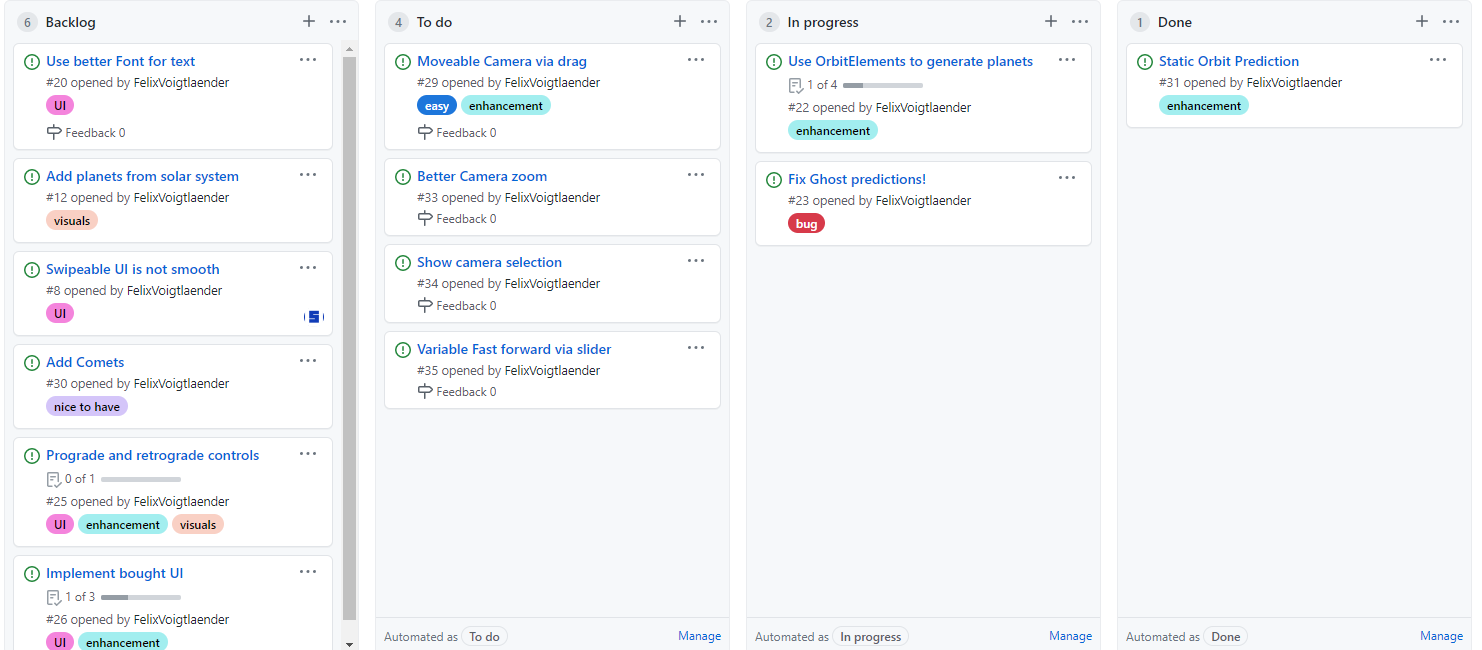
\includegraphics[width=1\textwidth]{Kanban.PNG}
      \caption{Example Kanban Board}
      \label{fig:kanban}
  \end{minipage}%
\end{figure}

The “Backlog” holds all tasks for the project which need to be done for the final product. New tasks may be added for new features, 
bugs or changes. In each iteration tasks may be selected from the backlog and moved to the “todo” section.

The “todo” section holds all tasks which need to be completed and moved to the “done” section by the end of the current iteration. 
Thus tasks need to be selected such that the team is not over nor under burdened. New tasks shouldn’t be added from the backlog during 
an iteration, to keep the flow manageable and to avoid further issues. Once a task is being worked on it is moved to the “in progress” section.

The “in progress” section holds all tasks, which are being currently worked on. This section may also hold a review section to which 
tasks are moved once they are completed and to be tested and reviewed. Finally the completed tasks are moved to the “done” section.

The “done” section holds all tasks which are completed.

In this example at the beginning of each iteration tasks are selected from the “backlog” section and moved to the “todo” section, 
these tasks should be completed by the end of this iteration. Developers can now pick their tasks and move them to the “in progress” 
section and work on them. Once the task is completed the developer can move their task to the “done” section, in case of a review section 
the developer moves the task to the “review” section instead, which will then be reviewed. In case of issues the task might be moved back 
to the “todo” section with a description of an issue or a bug report may be formulated.

In case the “in progress” section reaches its maximum number of tasks, new tasks from the todo list are not allowed to be moved to the 
“in progress” section. Instead, developers must complete their tasks before starting new ones and freed up developers can help others. 

The agile Kanban model is simple to understand and easy to manage. It visualizes the workflow clearly on a board, which 
is straightforward to read for people of different backgrounds. It enables the team to self manage task allocation decreasing 
the number of bottlenecks during development.

The model  is flexible and makes it easy to adapt to changes during development. It is consistent and easily measurable and always 
improvable, by altering structures, definitions, or tasks. Changes are gradual, making it easier for a team to adapt.

Yet clustered boards, with too many tasks or even outdated ones can lead to issues in development. Overcomplicating the model may 
also lead to slower development and communication. Overestimating or underestimating the workload, thus selecting the wrong amount and
types of tasks in each iteration leads to slower development and other issues like wasted resources and a clogged up pipeline.

In a nutshell, the Kanban model is a useful tool for workflow visualization and management. And if used correctly, thus the board is simple to read 
with correct iteration estimates, the board can be an effective tool for efficiency and self-improvement. The model is also very adaptable 
since at first only the board and iteration plannings need to be introduced, without having to change large portions of team structures.


\section{An Example}
In a student project\cite{ref_planeter} rapid prototyping has been used during development and for the creation of its user interface. 
The project aims to create an orbit based puzzle game on mobile devices with high influence from the desktop game 
Kerbal Space Programm. For the static orbit prediction of planets Keplerian elements and his laws of planetary motion
are used. The dynamic predictions for the user-controlled spaceship use a performance adapted gravity system approach
and simple Newtonian calculations. The project has been in development for 3 months and is aimed to release in 6 months.

For modularity, plasticity and rapid synthesis of prototypes the engine Unity has been used, which uses a component-based system 
and as scripting language C\# is used. In combination with rapid prototyping an altered version of the agile Kanban\cite{ref_kanban} model 
is used to ensure manageability throughout the project, see \figref{kanban}. Such alterations include setting the definition of sprints 
as the completion of tasks in the "Todo" section, instead of set time cycles of one week. 
Once all tasks of a sprint are completed a new prototype with the changes is distributed to users.
Additionally, once tasks start clogging up the workflow, those tasks are reevaluated and might be decomposed into new smaller tasks.
To reduce the risk of feature creeping three design pillars have been defined that need to be addressed and may not be contradicted by additional features or content. These design pillars are minimalism, education and gratification. Users are able to 
download the latest prototypes/builds from Google Drive\cite{ref_planeterProto} and sessions in which the user is observed while using the prototype are done.

This paper addresses the prototyping approach for developing the user interface during puzzle sequences.
The input options include the setting of thrust direction, thrust ignition, pausing and unpause, different 
time scale options, saving and loading, zoom and target of the camera, and leaving the puzzle sequence.
The interface displays the solar system, the current predicted orbit of spaceship and planets, thrust stages left, and the 
estimated prediction if the thrust is ignited.

\begin{figure}[!htb]
  \centering
  \begin{minipage}{.5\textwidth}
      \centering
      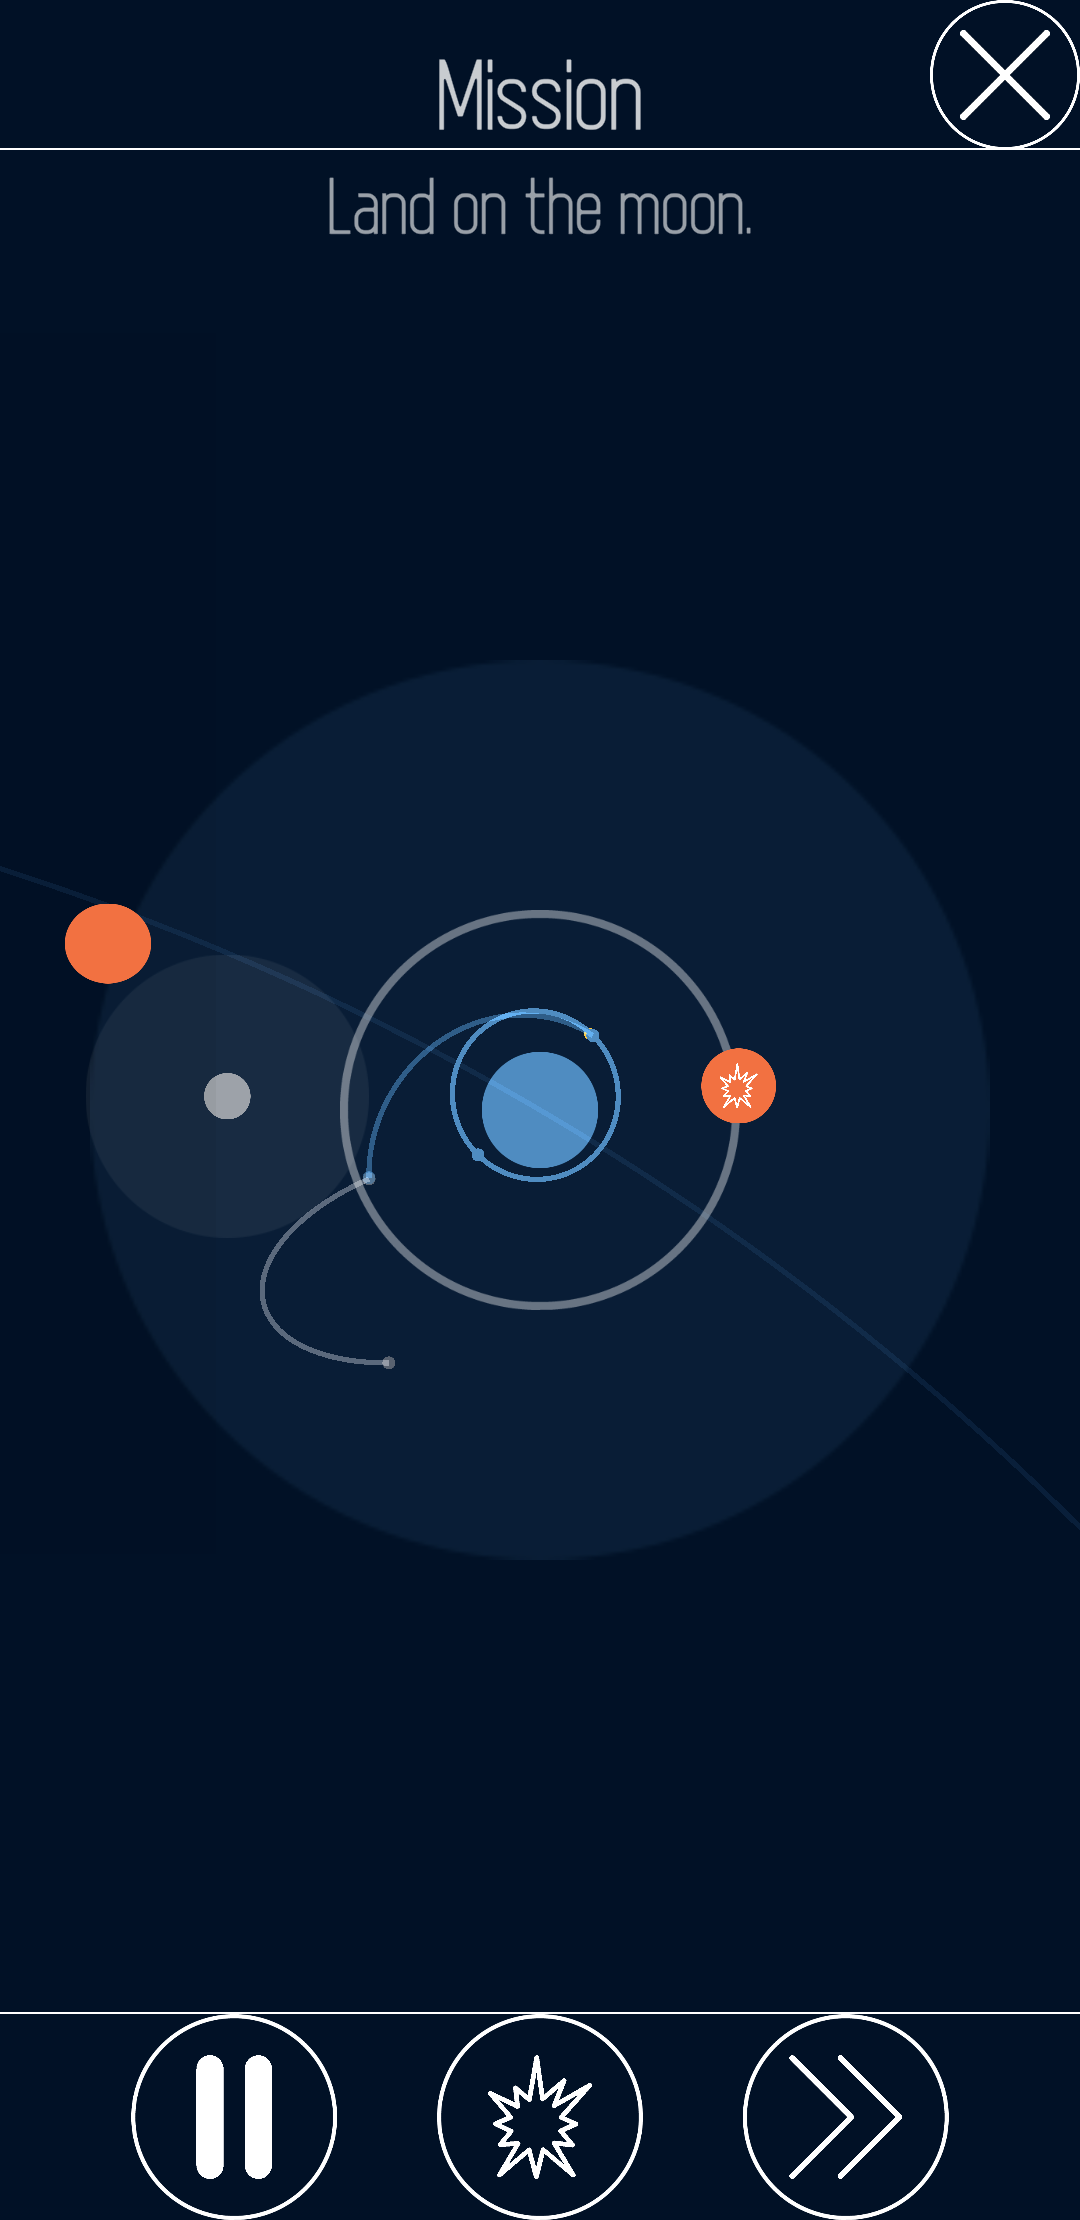
\includegraphics[width=0.8\textwidth]{Prototype1.png}
      \caption{Prototoype 1}
      \label{fig:prot1}
  \end{minipage}%
  \begin{minipage}{0.5\textwidth}
      \centering
      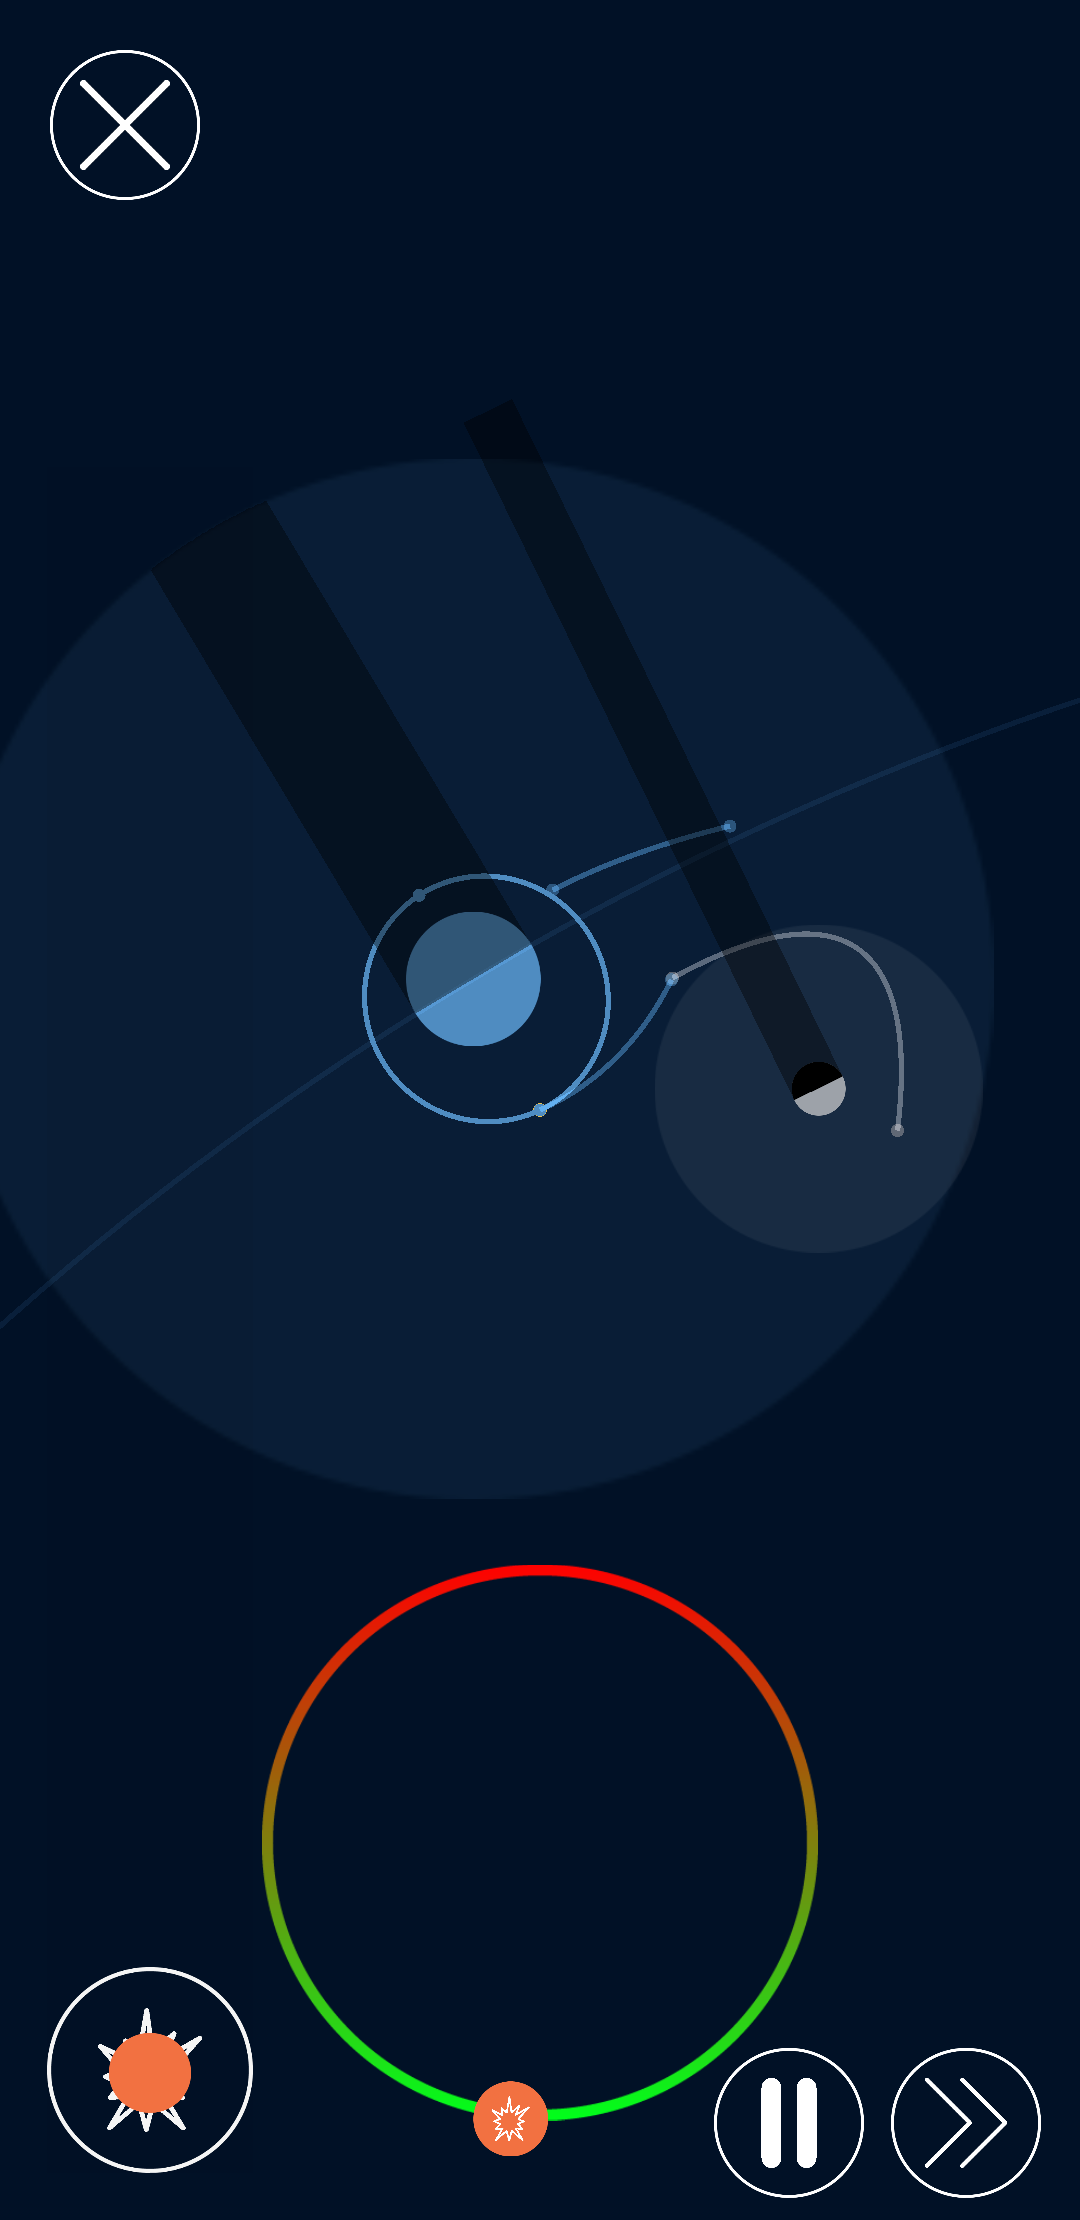
\includegraphics[width=0.8\textwidth]{Prototype2.png}
      \caption{Prototoype 2}
      \label{fig:prot2}
  \end{minipage}
\end{figure}

In the first initial prototype, see \figref{prot1}, the joystick for thrust direction is located at the center, a button for thrust
ignition is positioned at the bottom center next to pause/unpause and fast forward. Thrust stages are positioned at the middle
left.

The initial feedback by users was very helpful. It was pointed out that the user interface seems very cluttered, the orbit paths 
were hard to see and buttons did not show if the system was paused or not.

During observation of users interacting with the user interface more problems were discovered. At first most users clicked on the
staging, probably to ignite the stage, instead of the designated ignite button. Additionally some users accidentally clicked the
button to close the scenario. Also the joystick for thrust direction seemed to confuse some participants, especially during the simulation.

The second prototype, see \figref{prot2}, tries to address most issues. Unneeded lines and information has been removed or moved to the bottom 
or top of the screen, to declutter the user interface. The joystick for the thrust direction has been moved to the bottom center of the screen, with 
the addition to being relative to the velocity vector of the spaceship. Also staging and the ignition button have been moved to the 
same location, as to show which stage is ignited once pressed. The close button has been moved from right to left to address the issue of users accidentally closing the scenario.

Prototyping has been useful for the design of the user interface. Completely unknown issues, such as the staging and ignition button dependency,
have been discovered early in development and could be fixed without cost and time penalties, which would have been caused in later stages of development.

Additional feedback and observations from the second prototype have already been discovered. Such are the issue of multiple types of time scales, which
will be addressed via a slider for pause, normal time and several types of time scales. And additional issues with other user interface panels, relating
to this user interface panel.

Finally, prototyping has been helpful in finding and addressing issues found in user interface elements and system functions. This approach
will be used for further development.

\section{Conclusion}
Prototyping and Rapid Prototyping as tools for development can be useful to address the issues found in conventional methodologies if used correctly. 
It addresses the long development cycles, high development costs and assures customer and user satisfaction, due to their involvement
early and during development. Complex situations can be explored inexpensively with prototypes and iteratively improved.

Issues with prototyping need to be taken in consideration. Large systems are hard to prototype, user expectation needs to be managed and the 
management of projects using this approach is difficult.

But, in consideration of problems which might arise from prototyping and its advantages prototyping is a powerful tool for software and user interface
development.


%
% ---- Bibliography ----
%
% BibTeX users should specify bibliography style 'splncs04'.
% References will then be sorted and formatted in the correct style.
%
% \bibliographystyle{splncs04}
% \bibliography{mybibliography}
%
\begin{thebibliography}{8}

\bibitem{ref_prac}
Paul Beynon-Davies, Douglas Tudhope, Hugh Mackay: Information systems prototyping in practice. 
Journal of Information Technology  \textbf{14}(1), 107--120 (1999) 

\bibitem{ref_health}
R. Lenz, K.A. Kuhn: Towards a continuous evolution and adaptation of
information systems in healthcare. 
International Journal of Medical Informatics   \textbf{2004}(73), 75--89

\bibitem{ref_ui}
Dirk Bäumer, Walter R. Bischofberger, Horst Lichter, Heinz Züllighoven: User Interface Prototyping - Concepts, Tools, and Experience.
Proceedings - International Conference on Software Engineering 1996, DBLP \doi{10.1109/ICSE.1996.493447}

\bibitem{ref_IoTMethodologies}
Soukaina Merzouk, Abdessamad Cherkaoui, Abdelaziz Marzak, Saek Nawal: IoT methodologies: comparative study
International Workshop on Artificial Intelligence and Internet of Things (A2IoT) August 9-12, 2020, Leuven, Belgium

\bibitem{ref_RPInAction}
Toni Stokes Jones, Rita C. Richey: Rapid Prototyping Methodology in Action: A Developmental Study
ETR\&D, Vol.48, No. 2, 2000, pp. 63-80 ISSN 1042-1629

\bibitem{ref_RPalternativeStrategy}
Steven D Tripp, Barbara Bichelmeyer: Rapid Prototyping: An Alternative Instructional Design Strategy
ETR\&D Vol. 38, No. 1, pp. 31-44 ISSN 1042 1042-1629

\bibitem{ref_waterfall}
Dr. Winston W. Rovce: MANAGING THE DEVELOPMENT OF LARGE SOFTWARE SYSTEMS (1987)

\bibitem{ref_agilemanifesto}
The Agile Manifesto, \url{https://agilemanifesto.org/}. Last accessed 15
Nov 2020

\bibitem{ref_featurecreep}
Feature Creep, \url{https://www.agile-academy.com/de/agiles-lexikon/feature-creep/
}. Last accessed 15
Nov 2020

\bibitem{ref_kanban}
Eric Brechner: Agile Project Management with Kanban. Microsoft Press,
Redmond, Washington 98052-6399 (2015)

\bibitem{ref_planeter}
Student Project: Planeter, \url{https://github.com/FelixVoigtlaender/Planeter---Mini-Ksp
} Last accessed 14
Dec 2020

\bibitem{ref_planeterProto}
Student Project: Prototypes, \url{https://drive.google.com/drive/folders/1-CI-kAiKsY4FEDwQmcAWbDM9oTFoPtvh?usp=sharing} Last accessed 14
Dec 2020

\end{thebibliography} 
\end{document}
